\section{Power analysis calculations}
The calculation for the total energy cost for configuring the GrAICore and processing an input frame will be explained next.

\subsection{Configuration}
The configuration energy consists of the reading, transferring and writing of data from the external memory to the GrAICore's SRAMs. 

Let $C$ be the set of tuples holding the coordinates of every core:
\begin{equation}
    C = \{\,\left(x,y\right) \in \mathbb{N}^2 \mid 1 \leq x \leq 12 \wedge 0 \leq y \leq 11 \,\} 
\end{equation}

% \Cref{fig:model_data_heapmap} shows the amount of data from an arbitrary model that needs to be written to each of the 144 neuron cores.
\Cref{fig:model_data_heapmap} shows for a 80\% pruned version of ResNet-50\footnote{Internally named \texttt{resnet50\_pruned80\_star}} the amount of data that needs to be written to each of the 144 neuron cores.
We observe that the data is not uniformly distributed across the SRAMs.
Therefore, we require information how much data needs to be transferred to each SRAM.

\begin{figure}[hbtp]
    \centering
    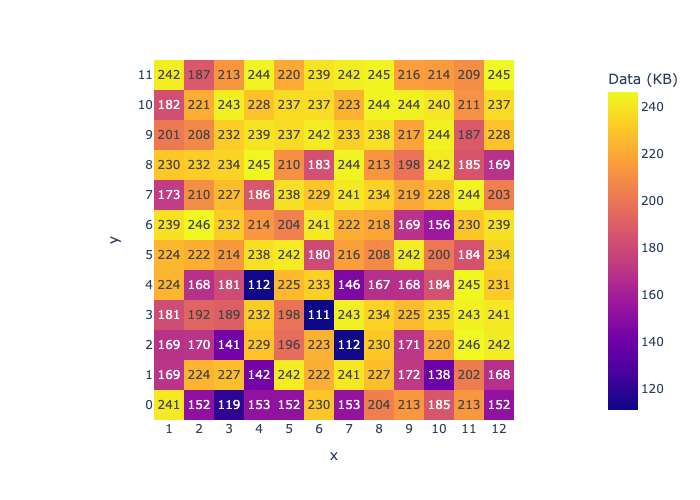
\includegraphics[width=0.8\linewidth]{assets/model_data_heatmap.png}
    \caption{Amount of data to be written to each core for the ResNet-50 model (80\% pruned).}
    \label{fig:model_data_heapmap}
\end{figure}

Let $D$ be a matrix of $12 \times 13$ with $D_{i,j}$ denoting the amount of bytes to be written to core $\left( i,j \right)$.
$D$ has an additional column due to the x-coordinates not starting from index $0$.
Its left-most column is unused (i.e., $D_{0,0}, D_{0,1}, \cdots, D_{0,11}$).
This matrix can be constructed from the artifacts outputted by the compiler.

The number of phits to be transferred through the config NoC influences the total energy costs.
In particular, the amount of phits to be transferred affects the number of hops to be taken in total and the amount of data to be written to the SRAMs.
Therefore, we need to determine how many phits needs to be transferred to each neuron core.
% The number of phits to be transferred influences the energy cost in the config NoC hops and SRAM writes.
% A packet can contain up to 520 bytes\footnote{$65 \times \frac{64}{8}$} of payload data. 
A packet can contain up to 65 data phits, that is $65 \times \SI{64}{b} = \SI{520}{B}$ of payload data.
% If we transfe
Suppose we need to transfer $d$ bytes to a neuron core, we then require a total of $\left\lfloor \frac{d}{520} \right\rfloor$ packets with 65 data phits.
% If $d \bmod 520 > 0$, then there is an additional packet consisting of $\left\lceil \frac{\left( d \bmod 520 \right) \times 8}{64}\right\rceil$ data phits.
If $\left( d \bmod 520 \right) > 0$, then there is an additional packet for the remaining $\left( d \bmod 520 \right)$ bytes of data.
The remaining packet will consist of $\left\lceil \frac{d \bmod 520}{8}\right\rceil$ data phits.
Note that each packet also contains a single phit of 64 bits for the header information.


The total energy cost for configuring the GrAICore can be estimated with the following equation:
\begin{equation}
    E_{\textrm{config}} = E_{\textrm{ext\_mem}} + E_{\textrm{noc}} + E_{\textrm{write}}
\end{equation}

With:
\begin{align*} 
E_{\textrm{ext\_mem}} &= 
        \sum_{c \in C}^{}{E_\textrm{read\_ext\_mem}(D_c) + E_{\textrm{send\_to\_noc}}(D_c)} \\
E_{\textrm{noc}} &=
    E_{\textrm{hop}} \times \sum_{c \in C}^{}{N_\textrm{hops}(c) \times p_{\textrm{total}}(D_c)} \\
E_{\textrm{write}} &=
    E_{\textrm{sram\_write\_64b}} \times \sum_{c \in C}^{}{p_{\textrm{data}}(D_c)}
\end{align*}

And:
\begin{align*} 
N_{\textrm{hops}}(x,y) &=
    \begin{cases} 
        x + y & \textrm{if } 0 \leq y \leq 5 \\
        x + y - 6 & \text{if } 6 \leq y \leq 11
    \end{cases}
\\
p_{\textrm{total}}(d) &=
    \left\lfloor \frac{d}{520} \right\rfloor \times (65 + 1) + \left\lceil \frac{d \bmod 520}{8} \right\rceil + 1 =
    \left\lceil \frac{d}{8} \right\rceil + \left\lfloor \frac{d}{520} \right\rfloor + 1 
\\
p_{\textrm{data}}(d) &=
    \left\lfloor \frac{d}{520} \right\rfloor \times 65 + \left\lceil \frac{d \bmod 520}{8} \right\rceil =
    \left\lceil \frac{d}{8} \right\rceil
\end{align*}

\begin{eqexpl}[15mm]
    \item{$p_{\textrm{total}}(D_c)$} total phits (includes headers) for transferring $D_c$ bytes
    \item{$p_{\textrm{data}}(D_c)$} total data phits (excludes headers) for transferring $D_c$ bytes
    \item{$N_{\textrm{hops}}(c)$} the amount of hops required to reach a neuron core at coordinate $c$, starting from the router closest to the injection point. It has two sub-functions due to the new config NoC's dual injector architecture
    \item{$E_{\textrm{read\_ext\_mem}}(D_c)$} energy for reading $D_c$ bytes from the external memory
    \item{$E_{\textrm{send\_to\_noc}}(D_c)$} energy for sending $D_c$ bytes from the external memory to the config NoC
    \item{$E_{\textrm{hop}}$} energy for performing a single hop in the config NoC
    \item{$E_{\textrm{sram\_write\_64b}}$} energy for writing back 64 bits to a neuron core's SRAM
\end{eqexpl}

\subsection{Processing}
The frame processing energy is the energy consumed when the GrAICore processes a single frame with a configured model.
The energy for processing a single input frame is approximated as follows:
\begin{equation}
    E_{\textrm{frame}} = \textrm{avg\_util} \times \textrm{cores\_used} \times \textrm{processing\_latency} \times \SI{21}{mW}
\end{equation}

These parameters can all be extracted from GrAIPEFRUIT simulation results.